\documentclass[a4paper,12pt]{letter}
\usepackage[czech]{babel}
\selectlanguage{czech}
\usepackage[utf8]{inputenc}
\usepackage{graphicx}
\usepackage{hyperref}
\hyphenation{vybor}
\begin{document}
\pagestyle{empty}
\begin{letter}{}{}
\begin{flushleft}
Otevřená města, z. s.\\ Malinovského náměstí 624/3\\ 602\ 00 Brno
\end{flushleft}
% \address{}
\date{V Brně dne 13.\ června 2017}

\opening{\textbf{Věc: Pozvánka na členskou schůzi}}

Zveme členy, zájemce o~členství i~ostatní příznivce na členskou schůzi, která
proběhne 29.\ června 2017 v~Brně. Členská schůze se uskuteční v~čase od 10:00 do
16:00 v~zasedací místnosti Podkova v~budově Magistrátu města Brna na adrese
Dominikánské náměstí\ 1. Vstup do zasedací místnosti je z~nádvoří (na obrázku
vpravo dole).

\begin{center} 
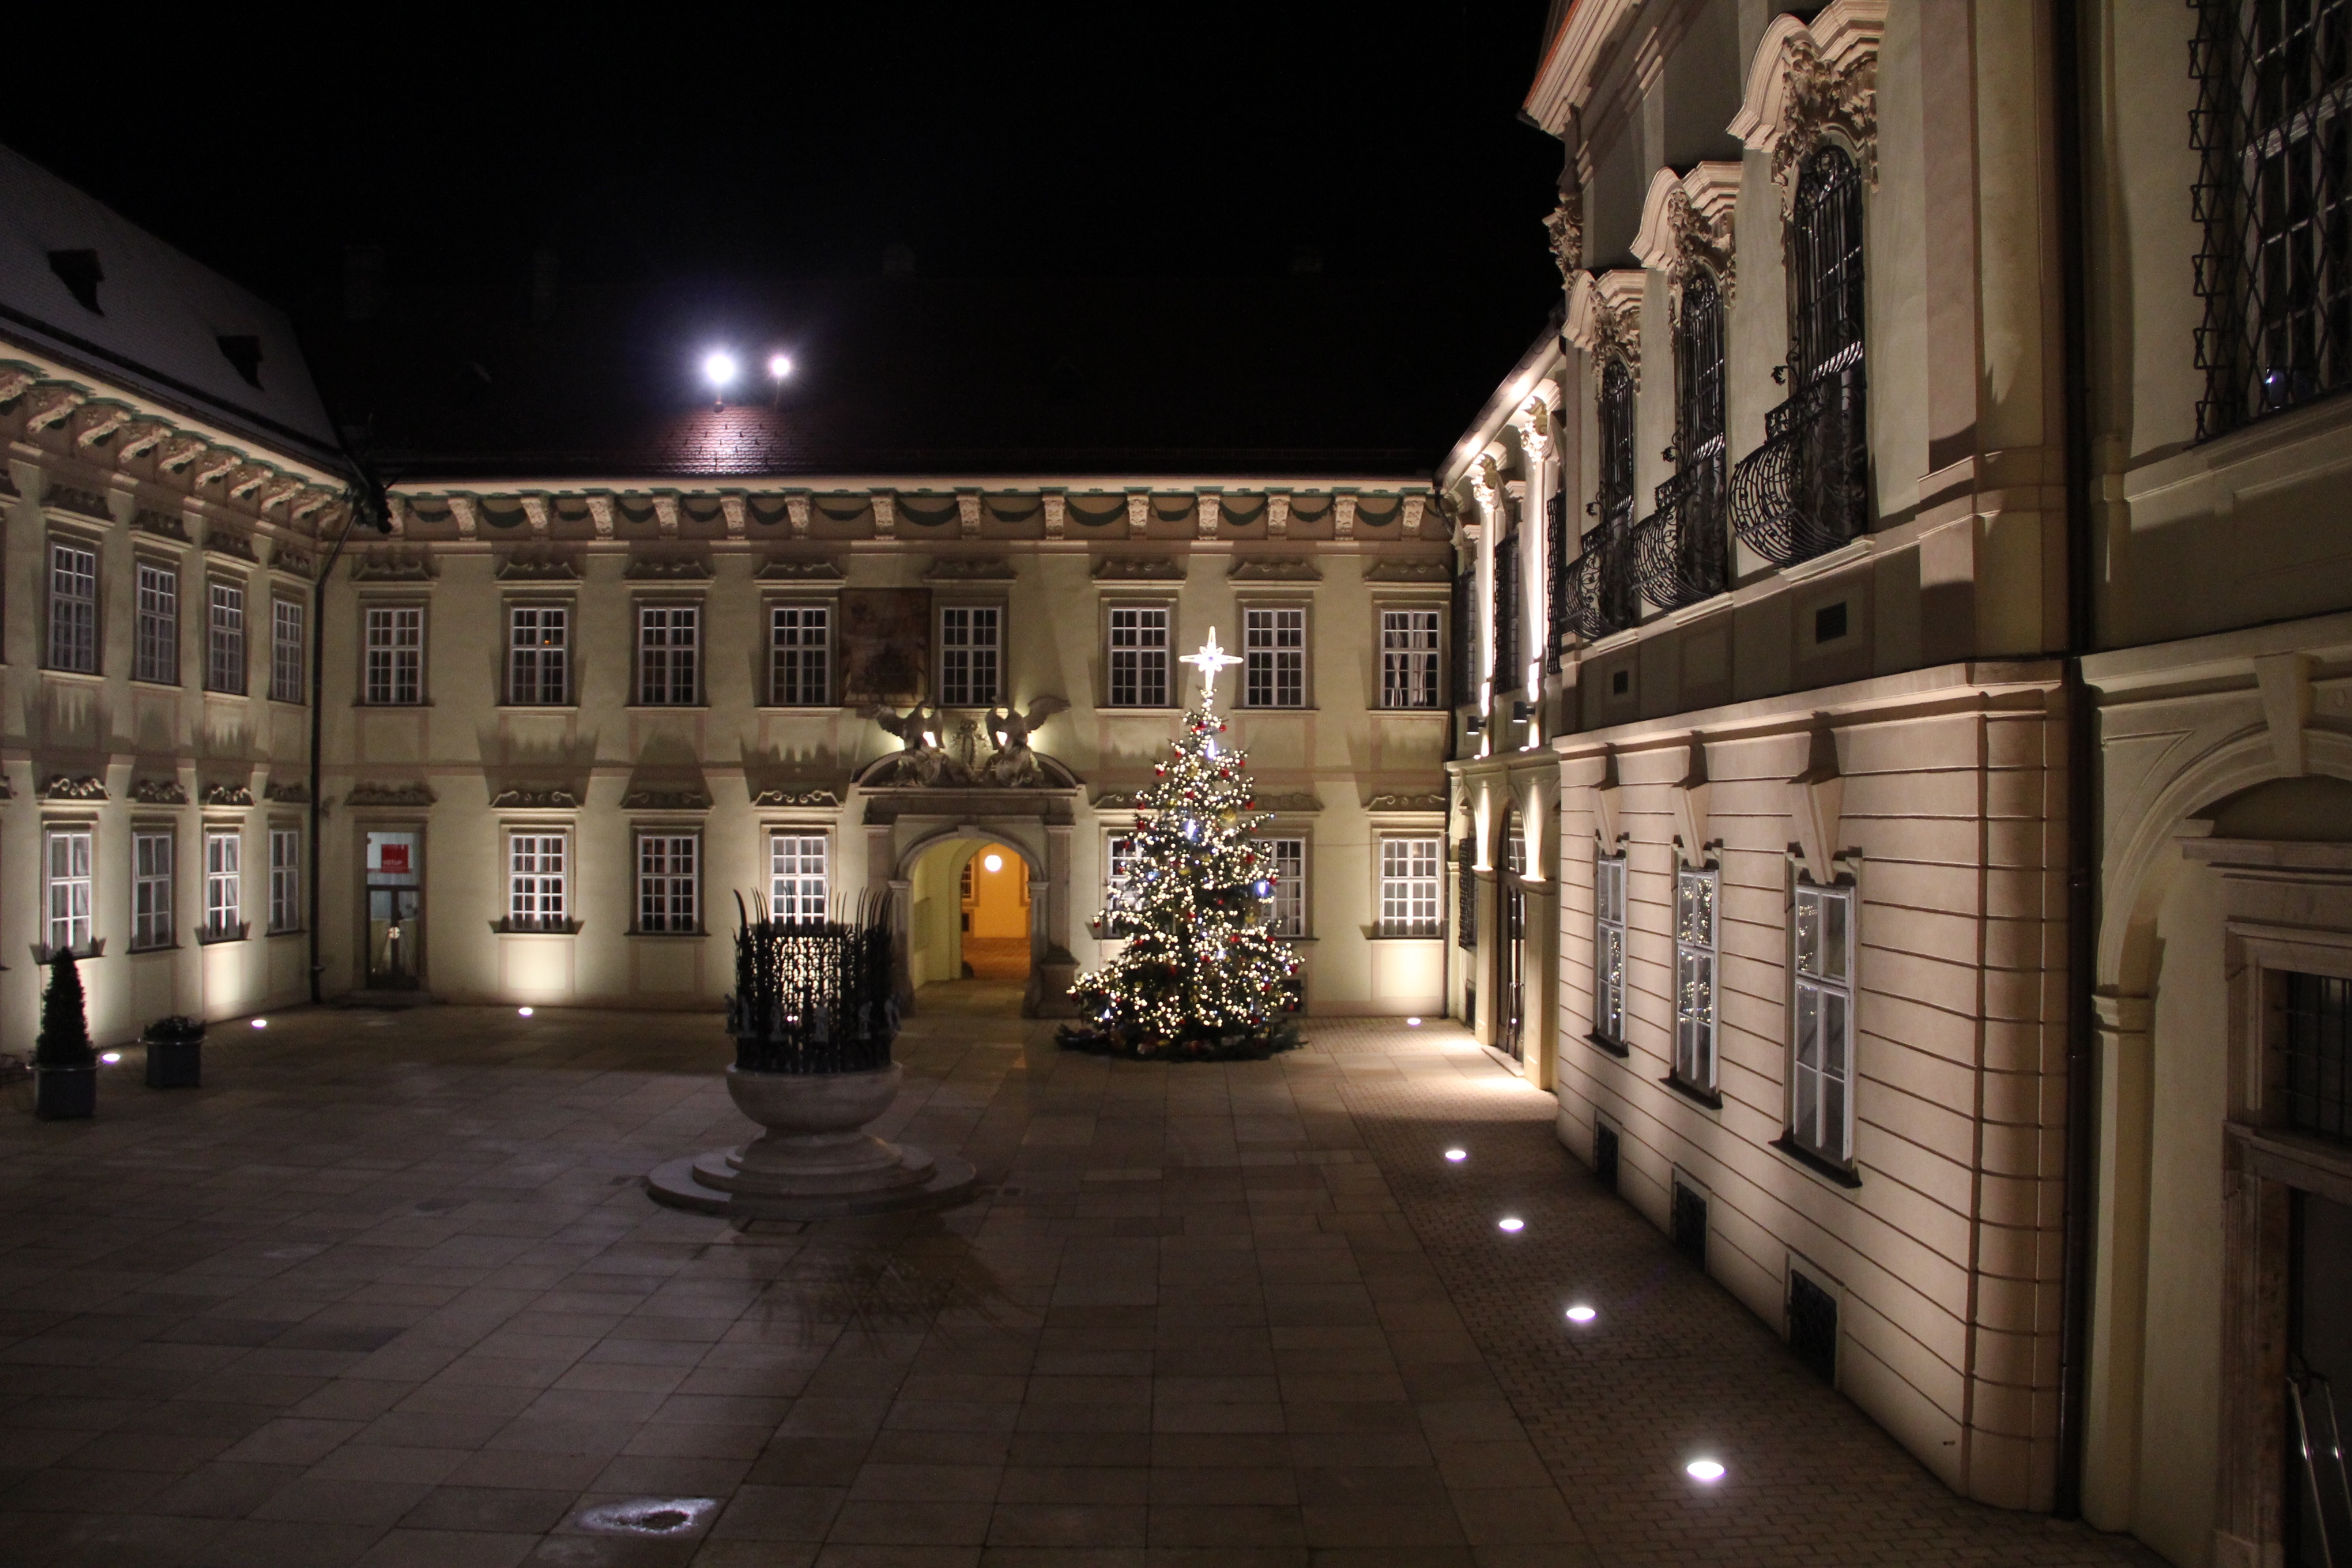
\includegraphics[width=0.9\textwidth]{Vecer_by_Niederkasseler_-_panoramio}\\
CC-BY-SA 3.0 Niederkasseler
\end{center} 

Členské schůze bude možné se účastnit také s~využitím videokonference
\emph{Jitsi Meet} na adrese
\href{https://meet.jit.si/OM-20170629}{https://meet.jit.si/OM-20170629}.
Vzdáleně bude možné hlasovat pouze pomocí textových zpráv z~mobilního telefonu.
Žádáme členy, kteří plánují účastnit se členské schůze vzdáleně, aby nám pro
účely hlasování na členské schůzi 29.\ června 2017 nejpozději do 20.\ června
2017 zaslali zprávou z~oficiálního účtu datových schránek člena číslo mobilního
telefonu, z~kterého bude zástupce člena hlasovat. Jiná forma vzdáleného
hlasování nebude možná. Rozhodnutí o~umožnění vzdáleného hlasování je vyhrazeno
členské schůzi.

Program členské schůze:

\begin{tabular}{rrp{0.5\textwidth}l}
číslo bodu & čas & bod & zpravodaj\\
& 8:00 & otevření místnosti & \\
& 9:15 & začátek registrace účastníků & \\
& 9:55 & konec registrace účastníků & \\
1 & 10:00 & schválení programu schůze & členové\\
2 & 10:10 & jednací řád členské schůze: vzdálená účast & Marcel Kolaja\\
3 & 10:20 & zpráva předsedy o činnosti (infrastruktura spolku, transparentnost
a zveřejňované informace, účetnictví, registr smluv, CityVizor, Open Source web
samosprávy, sdílení zkušeností, vystoupení na konferencích) & Marcel Kolaja\\
4 & 11:00 & priority projektů spolku pro následující období (revize existujícího
seznamu projektů, registr smluv a spolupráce se spolkem BISON, nové návrhy
členů) & Marcel Kolaja\\
5 & 12:30 & přestávka & \\
6 & 13:00 & tématické semináře/workshopy & členové\\
7 & 16:00 & ukončení\\
\end{tabular}

Také si dovolujeme upozornit na skutečnost, že hlasovat mohou pouze osoby, které
doložily nebo nejpozději na členské schůzi doloží své oprávnění zastupovat člena
na členské schůzi. Netýká se osob, které jsou zastupujícími dle Zákona o~obcích
(např. starosta, místostarosta, \ldots), nebo byly uvedeny v~usnesení
zastupitelstva.

Po ukončení členské schůze bude následovat afterparty. Pro účely organizace nám,
prosím, potvrďte předběžný zájem o~účast na afterparty. Dotazy směřujte na
e-mailovou adresu \href{mailto:vybor@otevrenamesta.cz}{vybor@otevrenamesta.cz}.

Seznam členů a jejich zástupců:
\begin{itemize}
\item Brno: Jiří Ulip
\item Brno-Medlánky: Kateřina Žurková
\item Brno-střed: Svatopluk Bartík
\item Černošice: Tomáš Kratochvíl
\item Česká Lípa: Tomáš Martínek
\item Kutná Hora: Lukáš Jelínek
\item Nove Město na Moravě: Michal Šmarda
\item Praha 5: Viktor Čahoj
\item Praha 7: Ondřej Profant
\item Praha-Ďáblice: Radimír Rexa
\item Psáry: Vít Olmr
\item Úvaly
\item EconLab: Jiří Skuhrovec
\item Frank Bold z.s.p.o.: Jiří Nezhyba
\item OpenAlt z.s.: Ladislav Nešněra
\item Oživení o.s.: Martin Kameník
\end{itemize}

\vspace{0.1\textwidth}
\begin{flushright}
\makebox[0.35\textwidth][l]{Marcel Kolaja,}\\
\makebox[0.35\textwidth][l]{předseda výboru,}\\
\makebox[0.35\textwidth][l]{\emph{Otevřená města, z. s.}}
\end{flushright}
\end{letter}
\end{document}
